\section{Localizar novos parceiros}

\par Esta busca permite ao usuário encontrar novos parceiros para compor a sua rede de relacionamentos. Para realizar esta busca, utilizou-se uma consulta muito semelhante a da funcionalidade anterior, acrescentando apenas o filtro para permitir a busca por nomes informado pelo usuário.

\par Para auxiliar o usuário nessa tarefa, foi criada uma nova consulta que leva em consideração apenas o nome do usuário, visando a sua localização independente de relacionamentos. Essa consulta é realizada apenas quando o número de resultados encontrados pelo nome informado pelo usuário for menor que um determinado valor definido, nesse caso, cinco.

\par A Figura~\ref{fig:busca_novos_parceiros} apresenta o resultado da busca por novos parceiros, contendo uma lista com as pessoas que atendam os requisitos pré estabelecidos na consulta.

\newpage
\begin{figure}[h!]
	\centerline{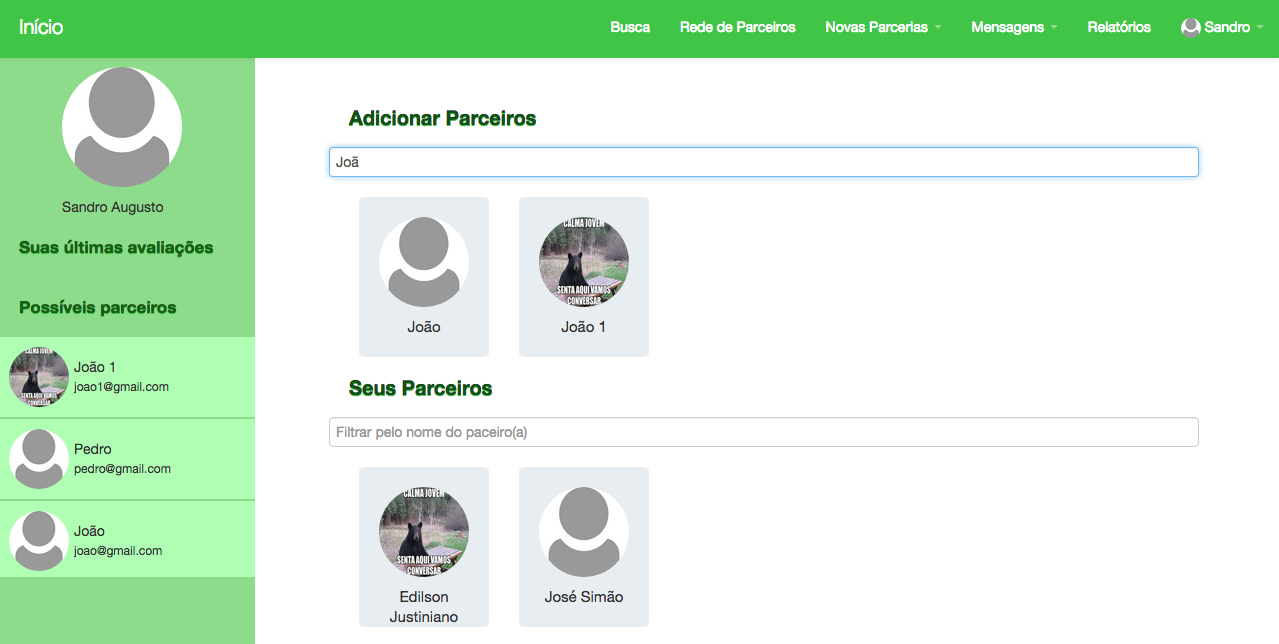
\includegraphics[scale=0.3]{./imagens/busca-novos-parceiros.png}}
	\caption[Funcionalidade que apresenta a busca por novos parceiros.]
	{Funcionalidade que apresenta a busca por novos parceiros. \textbf{Fonte:} Elaborado pelos autores.}
	\label{fig:busca_novos_parceiros}
\end{figure}

\par  Esta funcionalidade permite então que o usuário localize novos parceiros, que são indicados por ele e não sugeridos pelo sistema, como acontece na funcionalidade anterior.